\chapter{Evaluation}
\label{chap:evaluation}

In this chapter, we first go over the performance of the \gls{ocr} algorithms.
Then we compare the performance of the \gls{ocr} algorithms against human judgement.
Additionally, we investigate the feasibility of using recognized text from pristine images as ground truth.
Finally, we evaluate the performance of the \gls{ocr} algorithms on different quality levels of the HM and VTM codecs.

\section{Performance of Optical Character Recognition}
\label{sec:ocr_performance}

First, we evaluate the impact of different distortion types on \gls{ocr} performance by comparing the mean \gls{cer} for various quality levels.
This analysis is performed separately for EasyOCR and Tesseract \gls{ocr} to determine which performs better.

For the comparison, we plot the mean \gls{cer} with regards to the \gls{gt} on the y-axis against different quality levels on the x-axis.
We do this for all the distortion types.

\begin{figure}[h]
\centering
    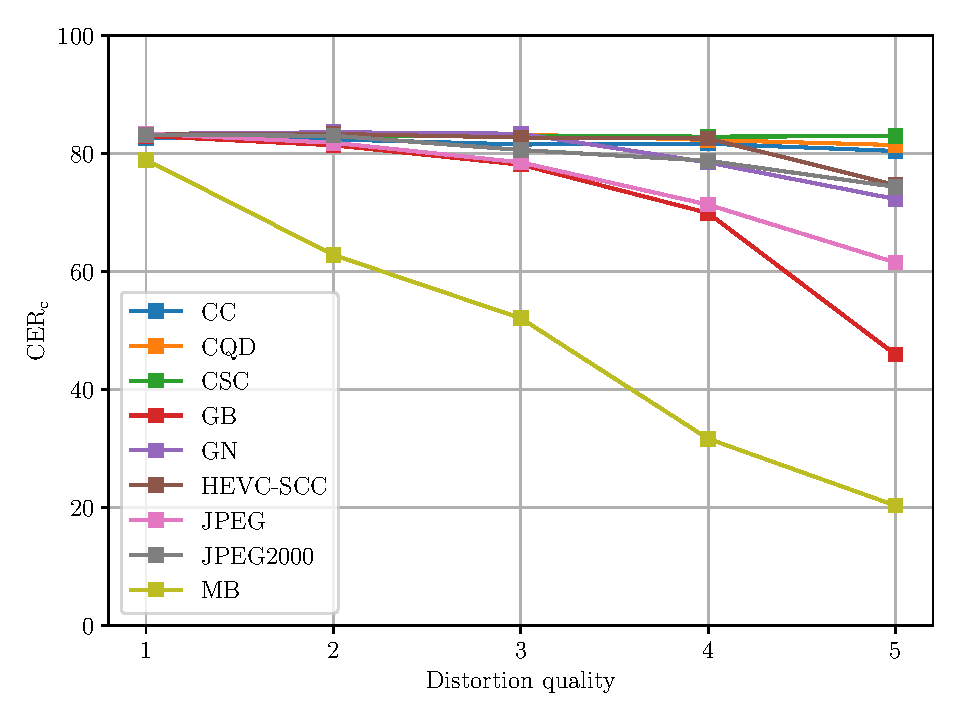
\includegraphics[width=0.9\textwidth]{../../images/analyze/cer_dist_quality_gt_ezocr.pdf}
    \caption{Mean \gls{cer} against \gls{gt} for different quality levels with EasyOCR.}
\label{fig:cer_dist_quality_gt_ezocr}
\end{figure}

In \autoref{fig:cer_dist_quality_gt_ezocr}, we observe the mean \gls{cer} in relation to the ground truth (\gls{gt}) for different quality levels using EasyOCR.
A noticeable trend is that motion blur has the most significant impact on EasyOCR's performance, exhibiting a nearly linear decrease from 80 to 20.
Both JPEG and Gaussian blur display similar behavior until quality level 4, after which Gaussian blur experiences a steeper decline.
Notably, the blurring of images greatly affects the legibility of text, with letters becoming indistinct and merging together, resulting in the poorest performance for EasyOCR.
Gaussian noise, JPEG2000, and HEVC-SCC exhibit comparable performance, all experiencing a decline at quality level 5.
The remaining distortions have minimal impact on performance, which is expected since color distortions do not directly affect text shapes.

\begin{figure}[h]
\centering
    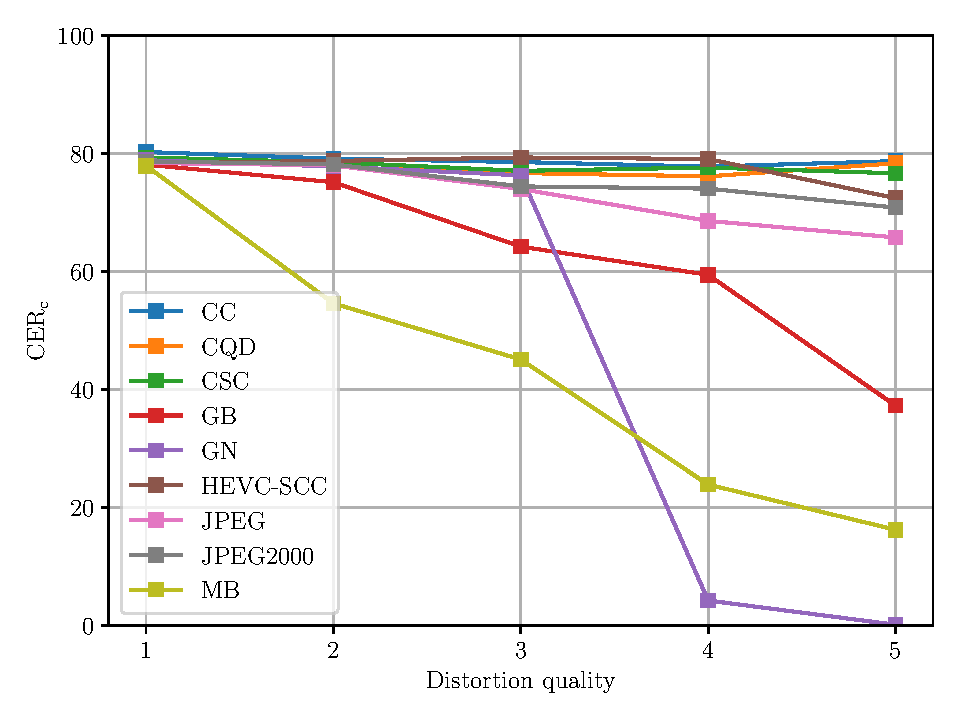
\includegraphics[width=0.9\textwidth]{../../images/analyze/cer_dist_quality_gt_tess.pdf}
    \caption{Mean \gls{cer} against \gls{gt} for different quality levels with Tesseract \gls{ocr}.}
\label{fig:cer_dist_quality_gt_tesseract}
\end{figure}

In \autoref{fig:cer_dist_quality_gt_tesseract}, we observe the mean \gls{cer} plotted in relation the ground truth (\gls{gt}) for various quality levels using Tesseract \gls{ocr}.
A steady decrease in \gls{cer} can be seen for motion blur and Gaussian blur, with the former exhibiting a 20-point higher value compared to the latter.
However, the most noteworthy finding is the significant drop in \gls{cer} for Gaussian noise at quality level 4, reaching 0 at quality level 5.
This sudden decline is particularly surprising when compared to other types of distortions.
Among the distortions analyzed, CC, CQD, and CSC perform the best, with CC even demonstrating a slightly higher \gls{cer} at quality level 5 compared to previous levels.
This phenomenon can possibly be attributed to CC's ability to enhance the distinction between the text and the background, acting almost like an image preprocessing step for the \gls{ocr}.
Interestingly, the \gls{cer} for HEVC-SCC slightly increases at quality level 4 and then decreases again at quality level 5.
A plausible explanation for this behavior is that certain portions of the text are not well recognized at quality 4, and since these unrecognized parts are not included in the \gls{gt}, it leads to a higher \gls{cer}.
Then at level 5, more parts, that are in the ground truth, are not recognized well.
Consequently, the \gls{cer} decreases.

In summary, our observations reveal that motion blur and Gaussian blur have a substantial impact on the performance of both EasyOCR and Tesseract \gls{ocr} algorithms.
Additionally, both \gls{ocr} algorithms perform demonstrate superior performance across images with CC, CQD, and CSC.
However, the most remarkable discovery is the significant drop in the \gls{cer} for Gaussian noise at quality level 4, reaching 0 at quality level 5, specifically for Tesseract OCR.
This suggests that EasyOCR exhibits greater robustness to Gaussian noise compared to Tesseract \gls{ocr} .
Overall, EasyOCR outperforms Tesseract \gls{ocr} , with a performance ceiling of approximately 83 \gls{cer} for EasyOCR, while Tesseract \gls{ocr} only achieves around 70 \gls{cer}.

\section{Comparison against human judgement}
\label{sec:comparison_against_human_judgement}

Available datasets with subjective quality scores will be utilized to investigate
the correlation between text recognition rates and human judgement.

\begin{itemize}
\item no clear correlation, ocr not getting substantially worse with worse quality \autoref{fig:sub29} and \autoref{fig:sub3}
\item transformation via fitted model might help
\end{itemize}

\begin{figure}[h]
\centering
    \includegraphics[width=0.9\textwidth]{../../images/analyze/mos_cer_ref_sub_mean_ezocr.pdf}
    \caption{Mean \gls{cer} against mean \gls{mos} for different reference images with EasyOCR.}
\label{fig:mos_cer_ref_sub_mean_ezocr}
\end{figure}

In \autoref{fig:mos_cer_ref_sub_mean_ezocr} we can see the mean \gls{cer} against the mean \gls{mos} over selected images for all distortions with EasyOCR.

\begin{figure}[h]
\centering
    \includegraphics[width=0.9\textwidth]{../../images/analyze/mos_cer_ref_sub_mean_tess.pdf}
    \caption{Mean \gls{cer} against mean \gls{mos} for different reference images with Tesseract \gls{ocr}.}
\label{fig:mos_cer_ref_sub_mean_tesseract}
\end{figure}

In \autoref{fig:mos_cer_ref_sub_mean_tesseract} we can see the mean \gls{cer} against the mean \gls{mos} over selected images for all distortions with Tesseract \gls{ocr}.


\begin{figure}[h]
\centering
    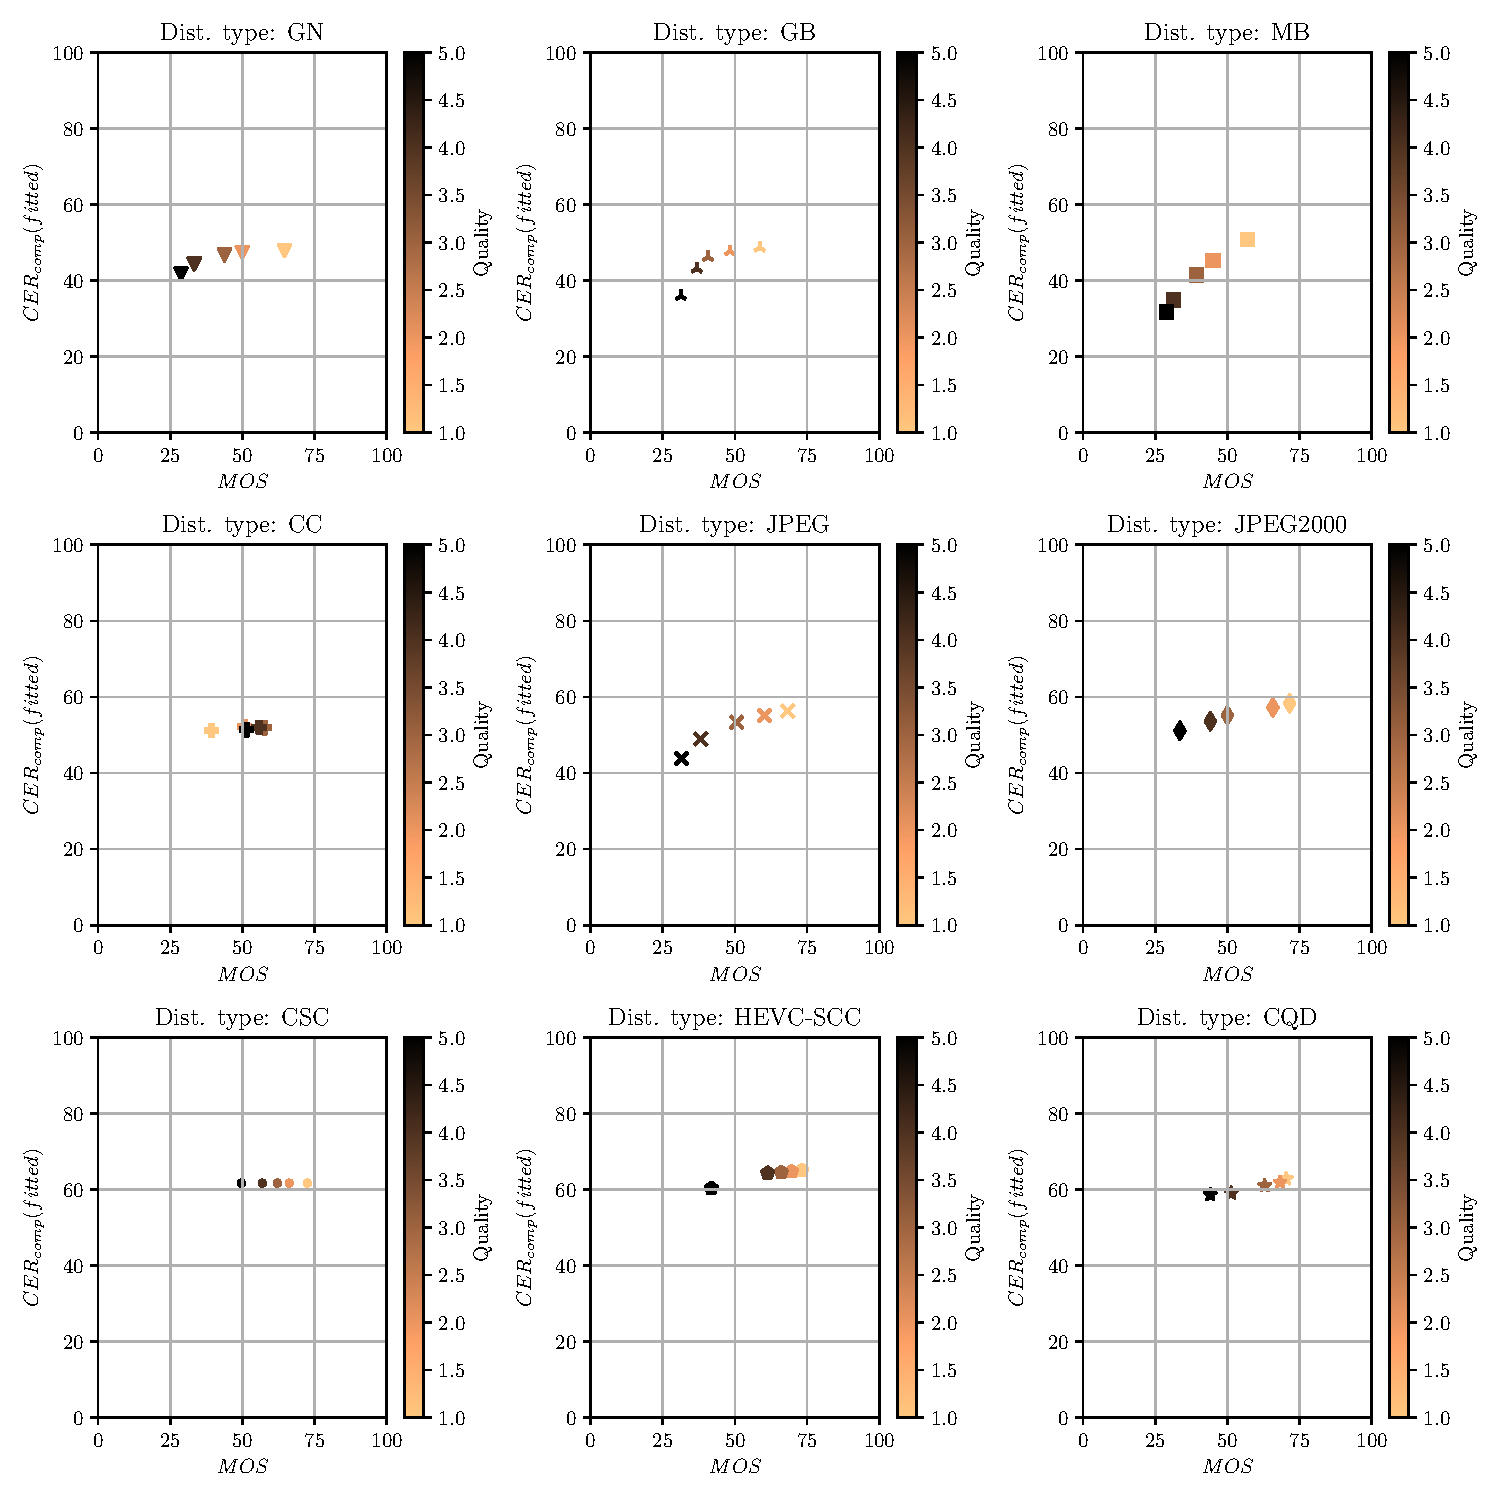
\includegraphics[width=0.9\textwidth]{../../images/analyze/mos_cer_ref_fitted_sub_mean_ezocr.pdf}
    \caption{Mean \gls{cer} (fitted) against mean \gls{mos} for different reference images with EasyOCR.}
\label{fig:mos_cer_ref_fitted_sub_mean_ezocr}
\end{figure}

In \autoref{fig:mos_cer_ref_fitted_sub_mean_ezocr} we can see the mean \gls{cer} (fitted) against the mean \gls{mos} over selected images for all distortions with EasyOCR.

\begin{figure}[h]
\centering
    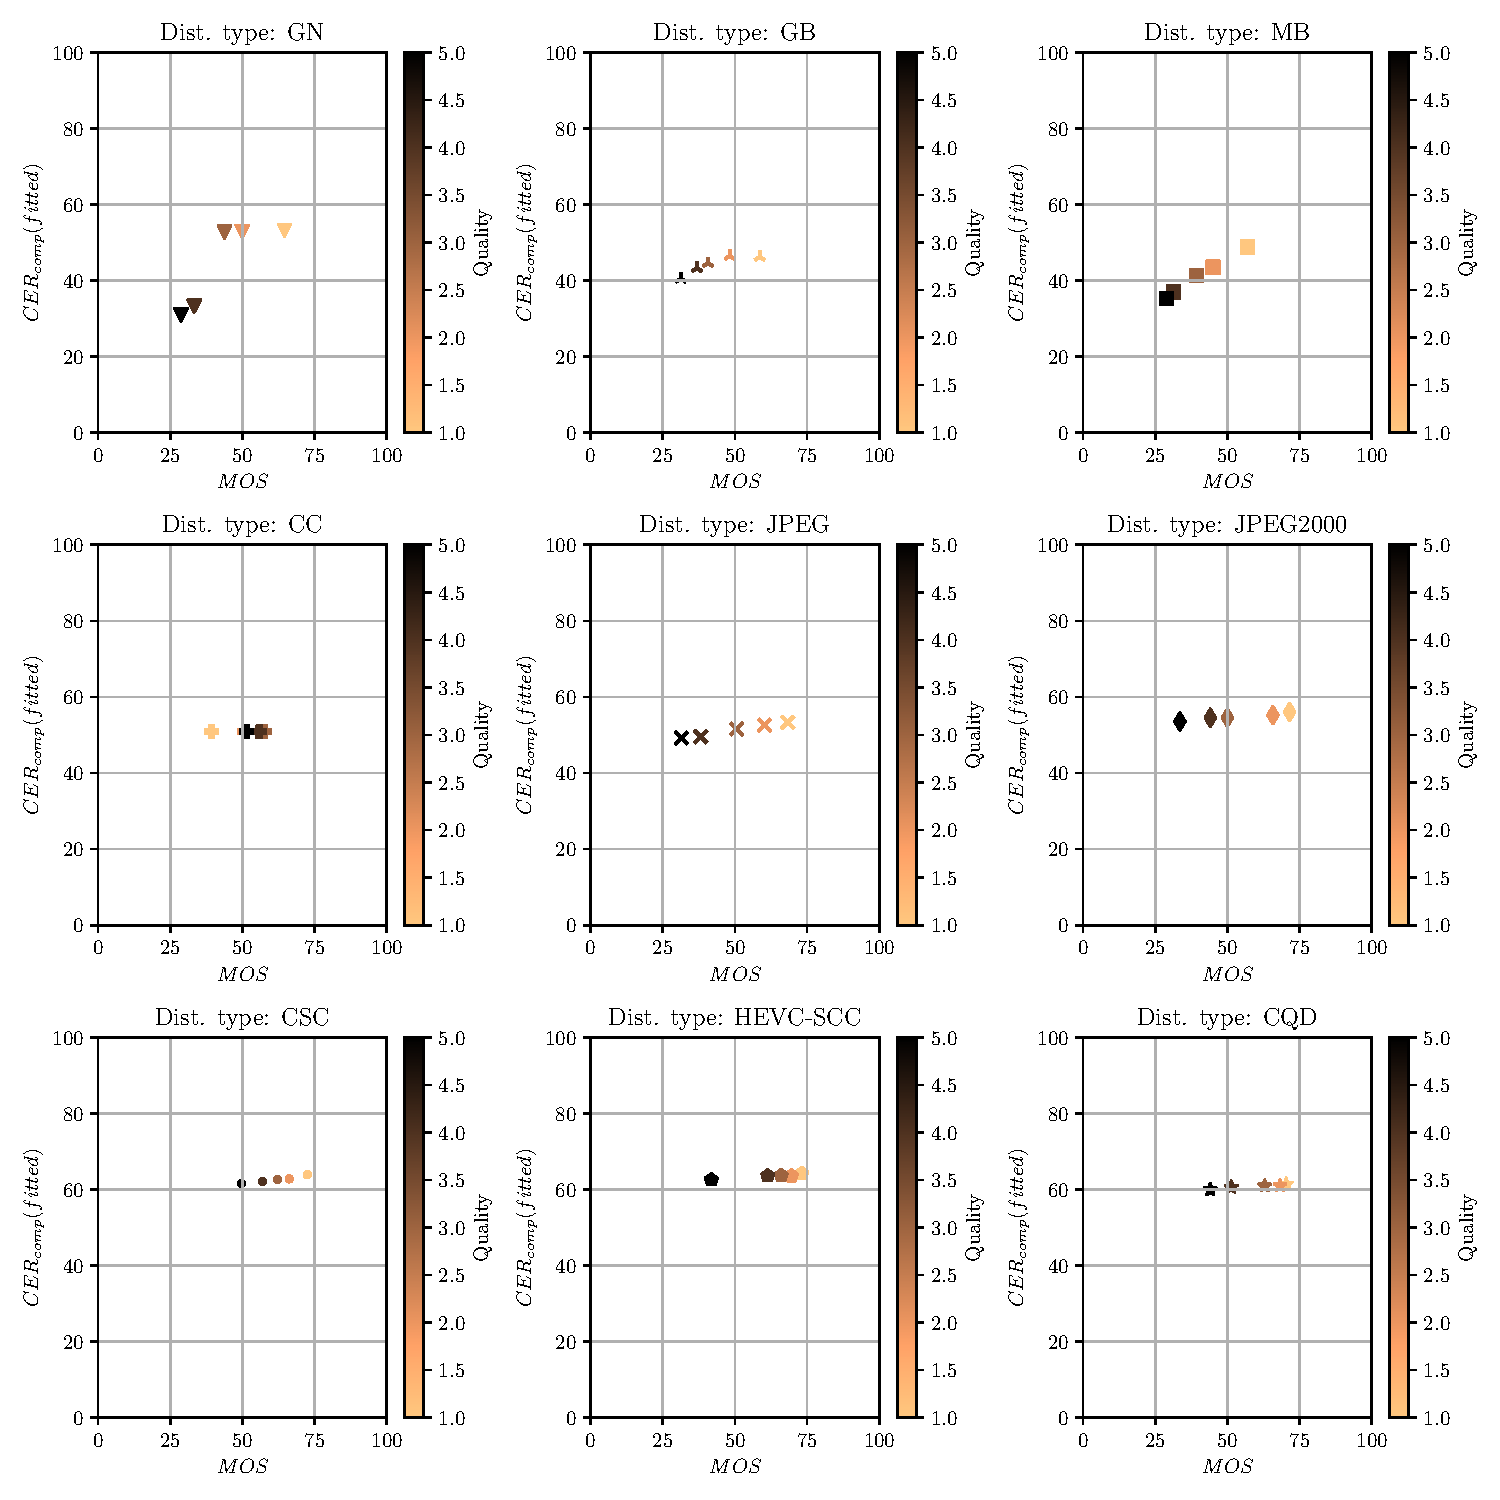
\includegraphics[width=0.9\textwidth]{../../images/analyze/mos_cer_ref_fitted_sub_mean_tess.pdf}
    \caption{Mean \gls{cer} (fitted) against mean \gls{mos} for different reference images with Tesseract \gls{ocr}.}
\label{fig:mos_cer_ref_fitted_sub_mean_tesseract}
\end{figure}

In \autoref{fig:mos_cer_ref_fitted_sub_mean_tesseract} we can see the mean \gls{cer} (fitted) against the mean \gls{mos} over selected images for all distortions with Tesseract \gls{ocr}.

\begin{table}[h]
\centering
\begin{tabular}{llrrrr}
\toprule
          & {} & \multicolumn{4}{l}{CER\_comp} \\
          & ocr\_algo & \multicolumn{2}{l}{ezocr} & \multicolumn{2}{l}{tess} \\
          & target &       \gls{gt} &   ref &    \gls{gt} &   ref \\
corr & dist\_name &          &       &       &       \\
\midrule
pearson & CC &     0.27 &  0.58 & -0.15 & -0.48 \\
          & CQD &     0.26 &  0.78 & -0.32 &  0.26 \\
          & CSC &    -0.06 &  0.73 &  0.08 &  0.13 \\
          & GB &     0.23 &  0.81 & -0.04 &  0.66 \\
          & GN &     0.32 &  0.83 &  0.87 &  0.88 \\
          & HEVC-SCC &     0.00 &  0.91 &  0.24 &  0.76 \\
          & JPEG &     0.74 &  0.89 &  0.56 &  0.83 \\
          & JPEG2000 &     0.02 &  0.89 &  0.45 &  0.59 \\
          & MB &     0.81 &  0.84 &  0.62 &  0.82 \\
spearmanr & CC &     0.22 &  0.42 & -0.18 & -0.58 \\
          & CQD &     0.23 &  0.79 & -0.44 &  0.27 \\
          & CSC &    -0.07 &  0.71 & -0.10 &  0.25 \\
          & GB &     0.46 &  0.94 &  0.08 &  0.61 \\
          & GN &     0.34 &  0.80 &  0.81 &  0.88 \\
          & HEVC-SCC &    -0.03 &  0.84 &  0.13 &  0.50 \\
          & JPEG &     0.70 &  0.98 &  0.56 &  0.81 \\
          & JPEG2000 &     0.09 &  0.95 &  0.35 &  0.63 \\
          & MB &     0.90 &  0.92 &  0.78 &  0.87 \\
\bottomrule
\end{tabular}
\caption{Correlation between CER\_comp and MOS for different distortion types}
\label{tab:pearson_spear}
\end{table}

\begin{table}[h]
\centering
\begin{tabular}{llrrrr}
\toprule
                 & {} & \multicolumn{4}{l}{CER\_comp\_fitted} \\
                 & ocr\_algo & \multicolumn{2}{l}{ezocr} & \multicolumn{2}{l}{tess} \\
                 & target &              \gls{gt} &   ref &    \gls{gt} &   ref \\
corr & dist\_name &                 &       &       &       \\
\midrule
pearson\_fitted & CC &            0.45 &  0.67 &  0.18 &  0.49 \\
                 & CQD &            0.52 &  0.75 &  0.32 &  0.34 \\
                 & CSC &            0.16 &  0.30 &  0.37 &  0.25 \\
                 & GB &            0.40 &  0.81 &  0.21 &  0.31 \\
                 & GN &            0.50 &  0.81 &  0.88 &  0.91 \\
                 & HEVC-SCC &           -0.01 &  0.85 &  0.16 &  0.09 \\
                 & JPEG &            0.72 &  0.92 &  0.81 &  0.86 \\
                 & JPEG2000 &            0.02 &  0.90 &  0.66 &  0.51 \\
                 & MB &            0.87 &  0.92 &  0.85 &  0.84 \\
spearmanr\_fitted & CC &            0.42 &  0.41 &  0.18 &  0.52 \\
                 & CQD &            0.38 &  0.79 &  0.06 &  0.33 \\
                 & CSC &            0.09 &  0.31 &  0.20 &  0.48 \\
                 & GB &            0.46 &  0.94 &  0.26 &  0.42 \\
                 & GN &            0.34 &  0.80 &  0.81 &  0.88 \\
                 & HEVC-SCC &           -0.03 &  0.84 &  0.25 &  0.19 \\
                 & JPEG &            0.70 &  0.98 &  0.75 &  0.81 \\
                 & JPEG2000 &            0.12 &  0.95 &  0.74 &  0.56 \\
                 & MB &            0.90 &  0.92 &  0.90 &  0.87 \\
\bottomrule
\end{tabular}
    \caption{Correlation between $CER_{comp}$ (fitted) and MOS for different distortion types}
\label{tab:pearson_spear_fitted}
\end{table}
    
\section{Usage of recognized text as ground truth}
\label{sec:usage_of_recognized_text_as_ground_truth}

Since most datasets do not contain textual ground truth information,
in a further step, Mr Hirt will investigate the feasibility of
using recognized text from pristine images as ground truth instead.

\begin{table}[h]
\centering
\begin{tabular}{|l|l|l|}
    \hline
    \rule{0em}{1em} \textbf{OCR Algorithm} & $\mathbf{\overline{CER}}$ & $\mathbf{\overline{CER}_{comp}}$ \\
    \hline
    EasyOCR & 0.16206 & 83.794 \\
    \hline
    Tesseract & 0.249047 & 75.0953 \\
    \hline
\end{tabular}
\caption{Mean $CER$ and $CER_{comp}$ for EasyOCR and Tesseract \gls{ocr} over selected images for reference images against \gls{gt}.}
\label{tab:mean_cer_cer_comp}
\end{table}

From \autoref{tab:mean_cer_cer_comp} we can see that EasyOCR performs better than Tesseract \gls{ocr} on the selected images.
With a $CER_{comp}$ of 83.794 its difficult to recommend using EasyOCR as a ground truth source.

\section{Codec comparison}
\label{sec:codec_comparison}

\begin{figure}[h]
    \centering
    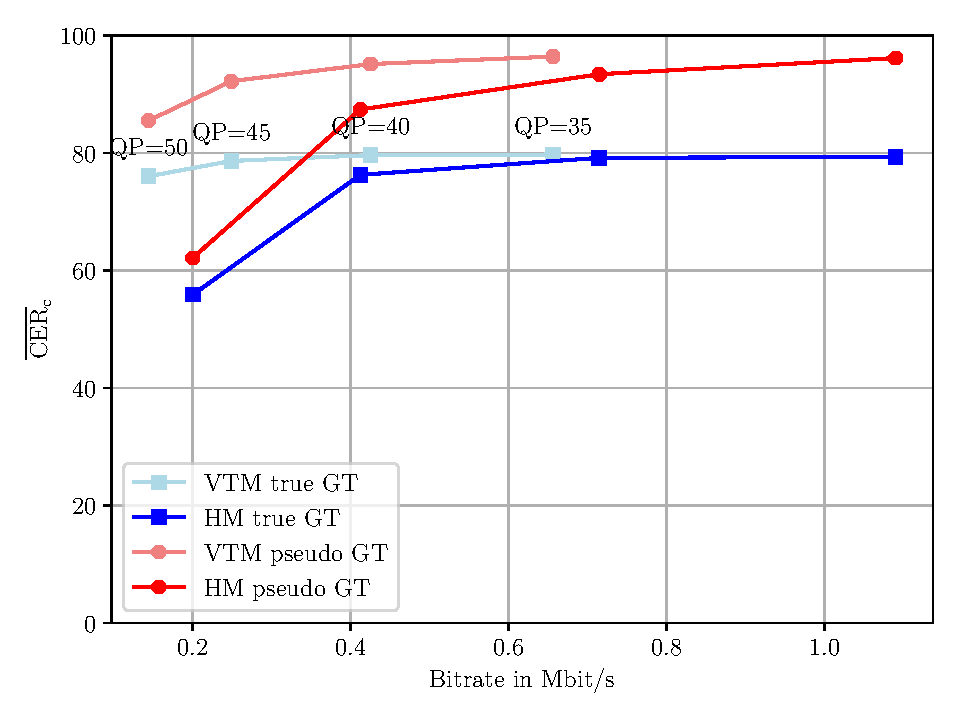
\includegraphics[width=0.9\textwidth]{../images/analyze/codec_cer_size_ezocr_default.pdf}
    \caption{Comparison of $CER_{comp}$ and size for HM and VTM codec for ezocr}
    \label{fig:codec_cer_size_ezocr_default}
\end{figure}

\begin{figure}[h]
    \centering
    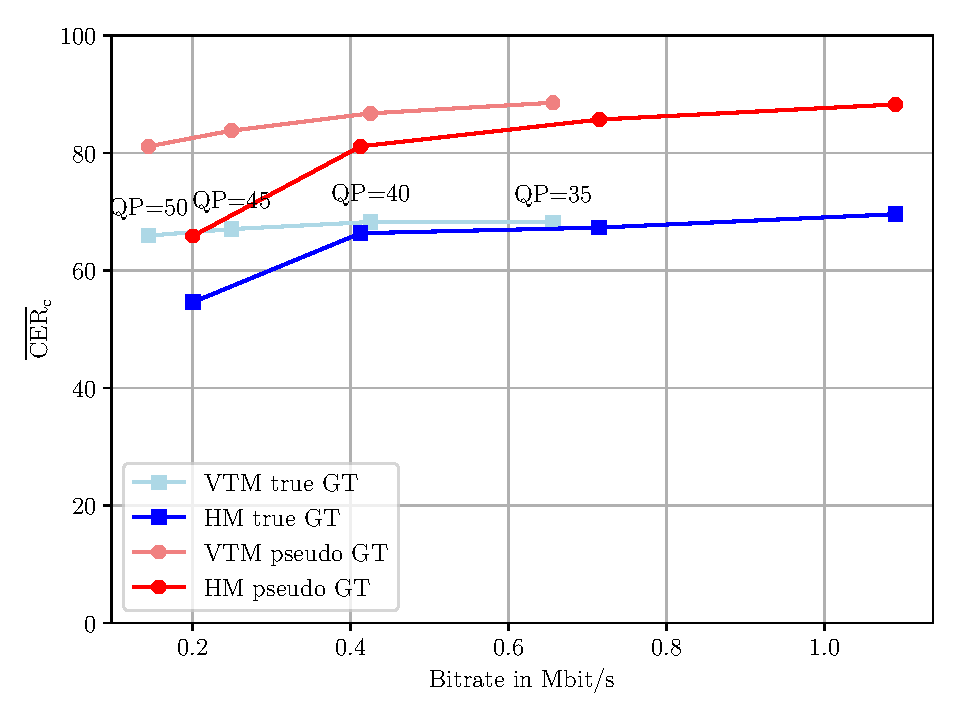
\includegraphics[width=0.9\textwidth]{../images/analyze/codec_cer_size_tess_default.pdf}
    \caption{Comparison of $CER_{comp}$ and size for HM and VTM codec for tess}
    \label{fig:codec_cer_size_tess_default}
\end{figure}

\begin{figure}[h]
    \centering
    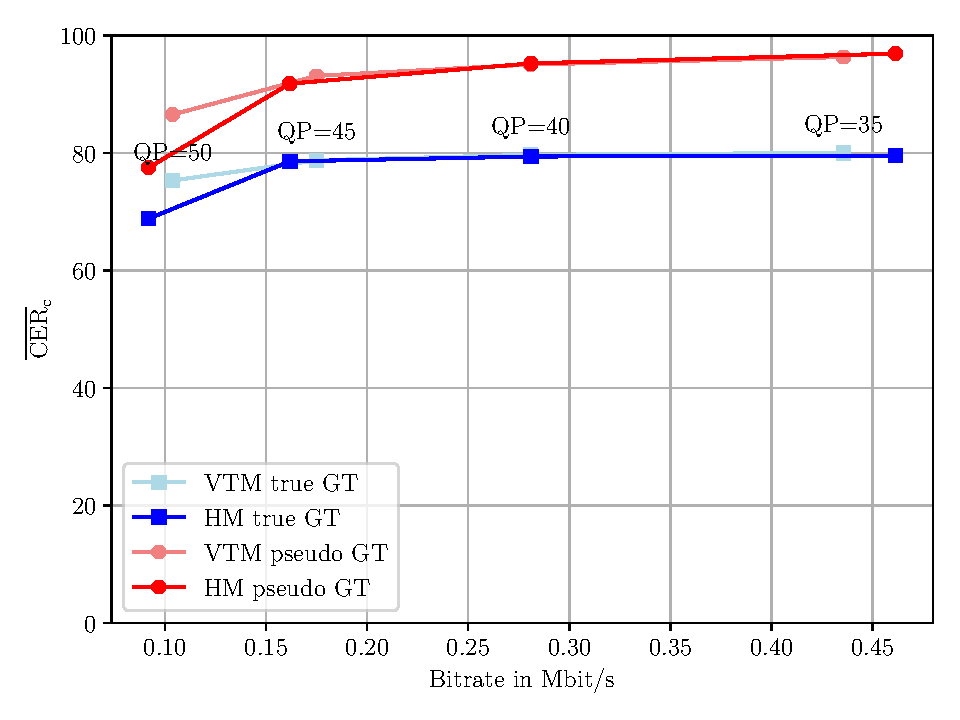
\includegraphics[width=0.9\textwidth]{../images/analyze/codec_cer_size_ezocr_scc.pdf}
    \caption{Comparison of $CER_{comp}$ and size for HM and VTM codec with SCC configuration for ezocr}
    \label{fig:codec_cer_size_ezocr_scc}
\end{figure}

\begin{figure}[h]
    \centering
    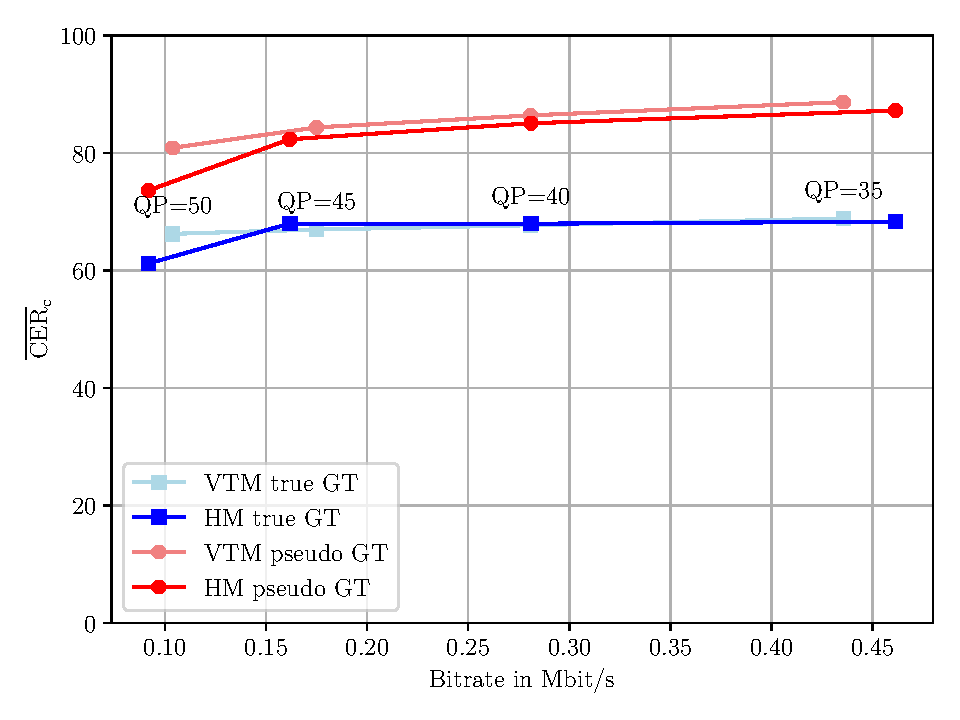
\includegraphics[width=0.9\textwidth]{../images/analyze/codec_cer_size_tess_scc.pdf}
    \caption{Comparison of $CER_{comp}$ and size for HM and VTM codec with SCC configuration for tess}
    \label{fig:codec_cer_size_tess_scc}
\end{figure}
